SyVOLT (Symbolic Verifier of mOdeL Transformations) is a user-friendly\markus{Do
we want to emphasize that the graphical editor is not yet really so great? At
least this is the feedback I got from some of my colleagues. We shoul not sell
this as ``the thing''.} Eclipse plugin to verify pre-/post- condition contracts
on model transformations specified in the DSLTrans transformation language. The
tool has a number of unique features, outlined below.

\subsection{Graphical Modelling of Model Transformation Contracts}

\markus{The first part of this subsection really isn't related to what the
subsection heading says. Maybe move this stuff above the subsection?} SyVOLT
proves that pre-/post-condition contracts hold for a model transformation. Such
contracts establish relations between patterns occurring in input and output
models of a model transformation. If a contract holds, then a formal guarantee
exists that whenever an input model contains the pattern specified in the
pre-condition of the contract, the output model contains the pattern specified
in the post-condition part of the contract and any traceability relations
between the two\markus{The part after ``and'' does not work grammatically.}.
Due to the graph-like structure of the pre and post conditions of contracts, the
visual representation of the contract in SyVolt editor allows the user to
quickly build and intuitively understand their meaning\markus{Only true to a
degree. The string concatenation syntax, for example, is really bad!}.
If a textual (logical or mathematical) editor where to be used, the user would
need an extra system of identifiers to correctly prescribe the associations
between pre and post-condition elements whereas in the visual representation,
the user graphically builds the associations between those elements\markus{That
part is certainly true. The story for he strings is different, though :-)}.
\levi{Claudio, I don't understand this sentence}
\cgg{Please tell me now if you can understand it.}
\markus{Looking at the other subsections here, I think this one really should
not be emphasized by being the first. Maybe having a subsection ``tool
support'' at the end? There you could also put the ATL stuff which I think is
out of place here; see below.}

The visual representation of a contract has all the necessary information to
derive the correct logical expression to be used by the internal SyVolt prover.

\subsection{Push-Button Proofs}
\label{sec:push_button_proofs}

SyVOLT is a verification tool that provides formal guarantees of correctness of
a model transformation\markus{Do we have to say this over and over again?}. The
proving process is fully automatic and the all formal details are completely
hidded from the user, who only needs to specify a set of contracts for the
transformation being verified. Once the transformation and the contracts of
interest are created, one command will start the property proving process. This
process will automatically create all required artifacts (as detailed in the
following section), run the process, and then provide the results to the user
within the Eclipse environment, as seen in Figure~\ref{fig:output}. This allows
the user to continually stay within the Eclipse environment, which is where he
develops the contracts and the model transformations.
\markus{Hmmm. Is it really about staying withing Eclipse? I think that, while
this is useful, the more important point is that the user stays on the
abstraction level of the contracts and properties, and is not exposed to low
level prover stuff.}


\subsection{Based on Symbolic Execution}

Our technique shares its principles\markus{What does this mean? Is it symbolic
Ex or not? If not, what exactly does it share and how is it different?} with
symbolic execution, a well-established code verification method.
The underlying idea entails building a finite representation of the (infinite)
set of model transformation computations, such that properties of interest can
be proved\markus{Check at the end: do we use proved and proven consistently?} on
such finite representation and extrapolated\markus{Sounds like this is not
safe. Use another word?} to the originally infinite set of possible
computations.

Our model transformation verification technique relies on typed graphs as the
means to internally represent both symbolic executions and contracts. SyVOLT
then reasons over these graphs to build a proof that contracts hold or do not
hold. Note that by using a typed graph representation, our technique can prove
contracts that include constraints on the attributes of the input and output
models. 

\levi{keep the text from here on?}\markus{If we use an example here, we should
also use one in the preceding sections. Otherwise remove.} An example of this
would be in the Families-To-Persons transformation from the ATL zoo [CITE]. In
this transformation, the name for a person in the output graph is a
concatenation of two strings \cgg{instead of ''strings``, should be
''attributes``}\markus{string values in attributes?} from elements in the input
graph. Our contract prover can prove that this concatenation will be valid in
all cases.

\begin{figure}
\centering
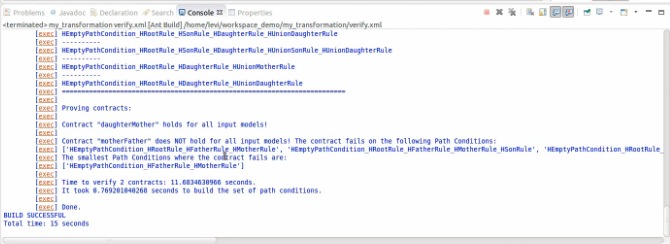
\includegraphics[width=0.45\textwidth]{figures/output}
\caption{The results of the contract prover}
\label{fig:output}
\end{figure}

\subsection{Input Independence and Exhaustiveness} 

Our technique is exhaustive, in the sense that whenever a contract holds, it
will hold for \emph{all} possible input models of a transformation. This is
possible because SyVOLT operates on specifications of outplace\markus{Is this a
word :-) ?} model transformations where unbounded loops and model element
deletions are not allowed. SyVOLT thus proves contracts in an input-independent
manner, relying only on the specification of the transformation itself. The
soundness and completeness of our technique is described in~\cite{Lucio2014}.

\subsection{Proving Contracts about ATL Model Transformations}

\markus{This section seems out of place; it does not describe anything about the
tool itself (like the other subsections) but rather a utility. Can this be moved
to some other place (or deleted, if it's not relevant to this paper)?} The Atlas
Transformation Language (ATL)~\cite{atlTool} is widely used in both industry and
academia. In order to extend our approach into these domains\markus{Which
domains? Academia and Industry???}, we have developed a higher-order
transformation that is able to automatically transform declarative ATL
transformations into our transformation language DSLTrans~\cite{Oakes}. This
allows the user to also prove contracts on ATL transformations.

\subsection{Performance and Scalability}
\markus{Changed speed to performance}

We have some evidence that SyVOLT scales to transformations of practical
interest. This has been empirically shown by applying it to DSLTrans
transformations up to over 60 rules, and ATL transformations up to 13
rules~\cite{Oakes}. From our own experience with DSLTrans, the size of a
DSLTrans transformations varies widely, with the average size ranging from 10 up
to 50 rules. The average size of an ATL transformation is around 20 rules. [cite
Manuel's paper, should we keep this?].\markus{Well, if we look at the case study
in this paper (mbeddr), then we can definitely see that to really verify mbeddr,
we'll have waaay more rules.} Even though our technique is exhaustive, our
approach takes relatively short amounts of time to prove contracts. For example,
our experiments with industrial transformations~\cite{Oakes} show that contracts
can be verified within a few minutes. In Gehan Selim's PhD
thesis~\cite{Selim2015} further evidence of SyVOLT's performance is given when
verifying a relatively large model transformation for giving semantics to the
UML-RT language in terms of the Kiltera process language~\cite{PosseDingel2014}.
SyVOLT's symbolic execution engine is fully
homegrown~\cite{LucioVang}\markus{Does ``homegrown'' have positive connotations?
Not sure.} and does not depend on third-party solvers. Although this has implied
a large effort to build the codebase, it has also allowed us to have the
required control over the code to iteratively optimize the engine for both space
and time economy.
\cite{Selim2014} demonstrates that our prover is substantially faster than
similar approaches based on SAT solvers.


\subsection{Production of Counter-Examples}

When a contract is proved to be violated by a given model transformation, it is
useful to also provide an input model -- called a \emph{counter-example} -- so
that the user can execute the model transformation with that input and verify
that indeed it violates the contract.\markus{The counter example is also used
to show an example. It doesn't literally have to be executed.}

An advantage of out technique is that the counter-example produced by SyVolt
describes a family\markus{How is it a family? Isn't it one example model?} of
input models that violate the contract.
This means that any input model that belongs to the family of the
counter-example -- i.e., fits the description given by the contract proving
process -- causes the model transformation to violate the contract. \cgg{Levi,
did you also show that any model that does not belong to the family does not
cause the model transformation to violate the contract?} Thus, the user can
easily determine the error in the transformation and correct it. We suggest that
this supports a transformation development method analogous to 'test-driven
development'. In this method, development would be routinely punctuated by
contract proof in order to catch errors early and store test cases -- the
counter examples produced -- to be used in the future.
\markus{I think you should mention that the notion of producing counter
examples is well established, eg in model checkers.}


\subsection{Integration with Eclipse}

\markus{Aha, ok, so you already have a paragraph abotu Eclipse. I suggest you
put the trafo editor here, together with the ATL stuff (ATL is also part of the
Eclipse ecosystem)} Eclipse is a popular development environment\markus{More
importantly, it is a platform for tool integration, in particular, for
model-based tools. This makes it really relevant for SyVOLT.} and model
transformation tools such as ATL~\cite{atlTool}, DSLTrans~\cite{Barroca2011} and
EGL~\cite{eglTool} are integrated with the Eclipse Modeling Framework
(EMF)~\cite{emfTool}.

To take advantage of this ecosystem, SyVOLT integrates with EMF\markus{Also
say something about Ecore?}.
In EMF, models can be represented in a multitude of syntaxes, from graphical
to textual, and this makes the interaction with SyVolt easier since the modeler
can use the model editor that is most convenient. Internally, SyVOLT uses 
the Himesis format~\cite{Provost2006} to represent models.

%\subsection{Model Driven Developed GUI\levi{this text is subsumed by section
%III a)}}
%\label{sec:mdd_gui}

%To take advantage of the productivity promised by MDD, we used a language
% called Eugenia[CITE] to develop the SyVolt contract editor shown in
%Figure~\ref{fig:eclipse_frontend}.
%With this approach, the SyVolt editor was developed in about 4 man-hours.

\begin{figure}
\centering
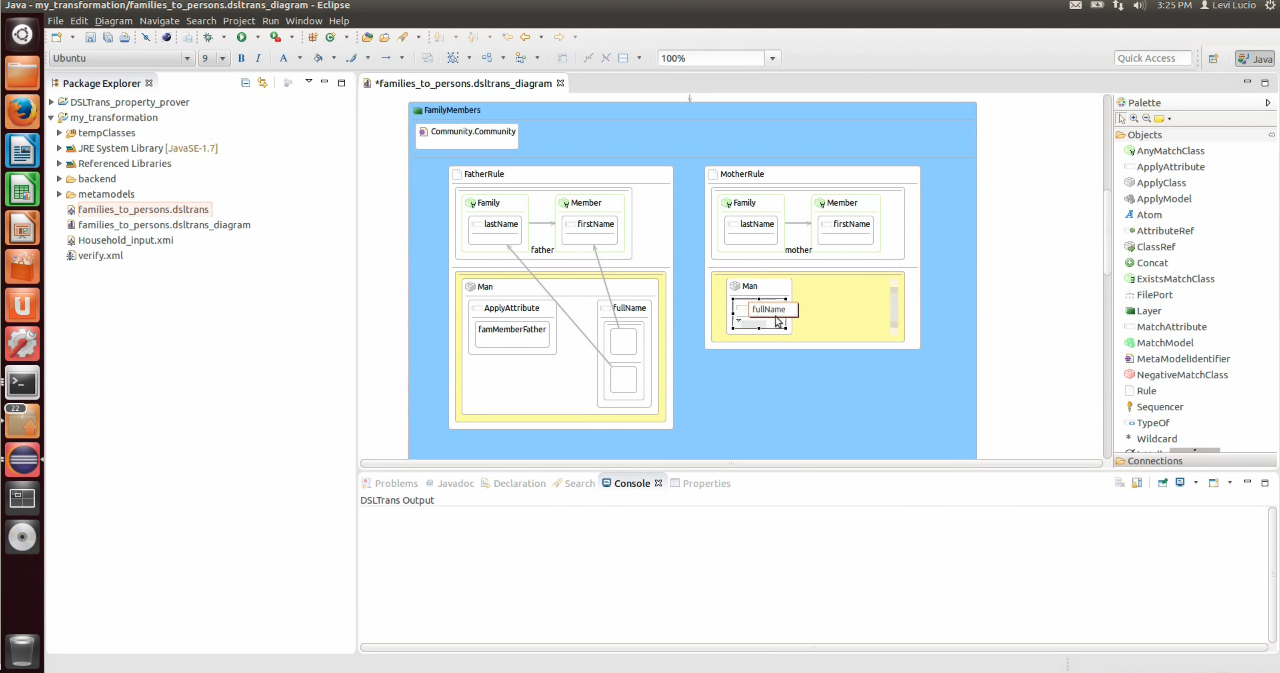
\includegraphics[width=0.45\textwidth]{figures/eclipse_frontend}
\caption{The transformation editor within Eclipse}
\label{fig:eclipse_frontend}
\end{figure}




 